
\subsubsection*{(100, 50) Window}

\begin{table}
    \caption{INRIA Results - (100, 50) Window}
    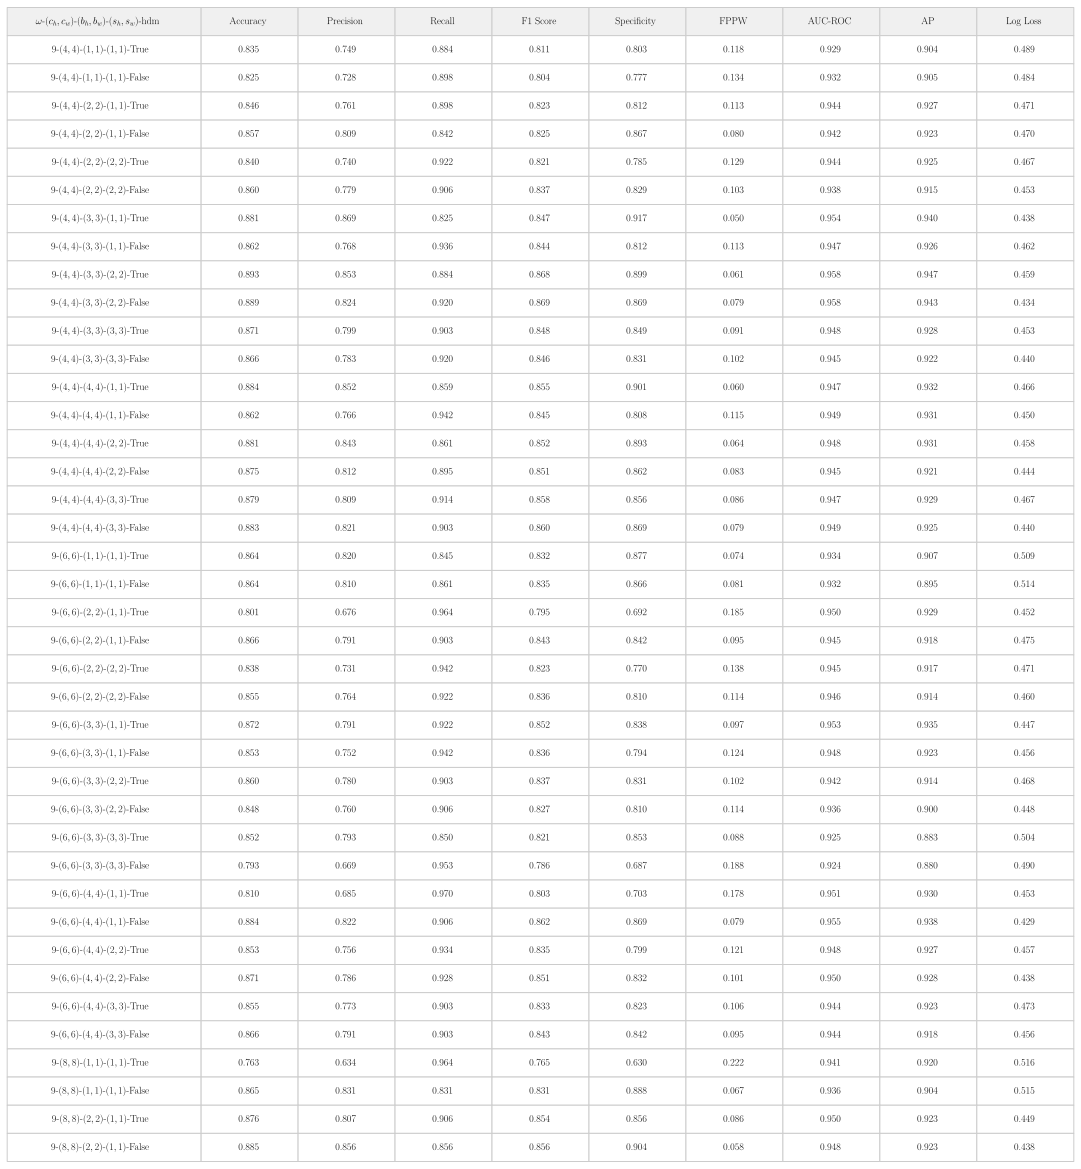
\includegraphics[width=\linewidth]{/Users/adamsam/repos/ib/ee/Pedestrian-Detection/code/paper/tables/INRIA/INRIA_(100, 50)_0.png}
    \label{tab:INRIA_(100, 50)_0}
\end{table}

\begin{table}
    \caption{INRIA Results - (100, 50) Window}
    \includegraphics[width=\linewidth]{/Users/adamsam/repos/ib/ee/Pedestrian-Detection/code/paper/tables/INRIA/INRIA_(100, 50)_120.png}
    \label{tab:INRIA_(100, 50)_120}
\end{table}

\begin{table}
    \caption{INRIA Results - (100, 50) Window}
    \includegraphics[width=\linewidth]{/Users/adamsam/repos/ib/ee/Pedestrian-Detection/code/paper/tables/INRIA/INRIA_(100, 50)_160.png}
    \label{tab:INRIA_(100, 50)_160}
\end{table}

\begin{table}
    \caption{INRIA Results - (100, 50) Window}
    \includegraphics[width=\linewidth]{/Users/adamsam/repos/ib/ee/Pedestrian-Detection/code/paper/tables/INRIA/INRIA_(100, 50)_200.png}
    \label{tab:INRIA_(100, 50)_200}
\end{table}

\begin{table}
    \caption{INRIA Results - (100, 50) Window}
    \includegraphics[width=\linewidth]{/Users/adamsam/repos/ib/ee/Pedestrian-Detection/code/paper/tables/INRIA/INRIA_(100, 50)_40.png}
    \label{tab:INRIA_(100, 50)_40}
\end{table}

\begin{table}
    \caption{INRIA Results - (100, 50) Window}
    \includegraphics[width=\linewidth]{/Users/adamsam/repos/ib/ee/Pedestrian-Detection/code/paper/tables/INRIA/INRIA_(100, 50)_80.png}
    \label{tab:INRIA_(100, 50)_80}
\end{table}

\subsubsection*{(112, 48) Window}

\begin{table}
    \caption{INRIA Results - (112, 48) Window}
    \includegraphics[width=\linewidth]{/Users/adamsam/repos/ib/ee/Pedestrian-Detection/code/paper/tables/INRIA/INRIA_(112, 48)_0.png}
    \label{tab:INRIA_(112, 48)_0}
\end{table}

\begin{table}
    \caption{INRIA Results - (112, 48) Window}
    \includegraphics[width=\linewidth]{/Users/adamsam/repos/ib/ee/Pedestrian-Detection/code/paper/tables/INRIA/INRIA_(112, 48)_120.png}
    \label{tab:INRIA_(112, 48)_120}
\end{table}

\begin{table}
    \caption{INRIA Results - (112, 48) Window}
    \includegraphics[width=\linewidth]{/Users/adamsam/repos/ib/ee/Pedestrian-Detection/code/paper/tables/INRIA/INRIA_(112, 48)_160.png}
    \label{tab:INRIA_(112, 48)_160}
\end{table}

\begin{table}
    \caption{INRIA Results - (112, 48) Window}
    \includegraphics[width=\linewidth]{/Users/adamsam/repos/ib/ee/Pedestrian-Detection/code/paper/tables/INRIA/INRIA_(112, 48)_200.png}
    \label{tab:INRIA_(112, 48)_200}
\end{table}

\begin{table}
    \caption{INRIA Results - (112, 48) Window}
    \includegraphics[width=\linewidth]{/Users/adamsam/repos/ib/ee/Pedestrian-Detection/code/paper/tables/INRIA/INRIA_(112, 48)_40.png}
    \label{tab:INRIA_(112, 48)_40}
\end{table}

\begin{table}
    \caption{INRIA Results - (112, 48) Window}
    \includegraphics[width=\linewidth]{/Users/adamsam/repos/ib/ee/Pedestrian-Detection/code/paper/tables/INRIA/INRIA_(112, 48)_80.png}
    \label{tab:INRIA_(112, 48)_80}
\end{table}

\subsubsection*{(128, 64) Window}

\begin{table}
    \caption{INRIA Results - (128, 64) Window}
    \includegraphics[width=\linewidth]{/Users/adamsam/repos/ib/ee/Pedestrian-Detection/code/paper/tables/INRIA/INRIA_(128, 64)_0.png}
    \label{tab:INRIA_(128, 64)_0}
\end{table}

\begin{table}
    \caption{INRIA Results - (128, 64) Window}
    \includegraphics[width=\linewidth]{/Users/adamsam/repos/ib/ee/Pedestrian-Detection/code/paper/tables/INRIA/INRIA_(128, 64)_120.png}
    \label{tab:INRIA_(128, 64)_120}
\end{table}

\begin{table}
    \caption{INRIA Results - (128, 64) Window}
    \includegraphics[width=\linewidth]{/Users/adamsam/repos/ib/ee/Pedestrian-Detection/code/paper/tables/INRIA/INRIA_(128, 64)_160.png}
    \label{tab:INRIA_(128, 64)_160}
\end{table}

\begin{table}
    \caption{INRIA Results - (128, 64) Window}
    \includegraphics[width=\linewidth]{/Users/adamsam/repos/ib/ee/Pedestrian-Detection/code/paper/tables/INRIA/INRIA_(128, 64)_200.png}
    \label{tab:INRIA_(128, 64)_200}
\end{table}

\begin{table}
    \caption{INRIA Results - (128, 64) Window}
    \includegraphics[width=\linewidth]{/Users/adamsam/repos/ib/ee/Pedestrian-Detection/code/paper/tables/INRIA/INRIA_(128, 64)_40.png}
    \label{tab:INRIA_(128, 64)_40}
\end{table}

\begin{table}
    \caption{INRIA Results - (128, 64) Window}
    \includegraphics[width=\linewidth]{/Users/adamsam/repos/ib/ee/Pedestrian-Detection/code/paper/tables/INRIA/INRIA_(128, 64)_80.png}
    \label{tab:INRIA_(128, 64)_80}
\end{table}

\subsubsection*{(128, 96) Window}

\begin{table}
    \caption{INRIA Results - (128, 96) Window}
    \includegraphics[width=\linewidth]{/Users/adamsam/repos/ib/ee/Pedestrian-Detection/code/paper/tables/INRIA/INRIA_(128, 96)_0.png}
    \label{tab:INRIA_(128, 96)_0}
\end{table}

\begin{table}
    \caption{INRIA Results - (128, 96) Window}
    \includegraphics[width=\linewidth]{/Users/adamsam/repos/ib/ee/Pedestrian-Detection/code/paper/tables/INRIA/INRIA_(128, 96)_120.png}
    \label{tab:INRIA_(128, 96)_120}
\end{table}

\begin{table}
    \caption{INRIA Results - (128, 96) Window}
    \includegraphics[width=\linewidth]{/Users/adamsam/repos/ib/ee/Pedestrian-Detection/code/paper/tables/INRIA/INRIA_(128, 96)_160.png}
    \label{tab:INRIA_(128, 96)_160}
\end{table}

\begin{table}
    \caption{INRIA Results - (128, 96) Window}
    \includegraphics[width=\linewidth]{/Users/adamsam/repos/ib/ee/Pedestrian-Detection/code/paper/tables/INRIA/INRIA_(128, 96)_200.png}
    \label{tab:INRIA_(128, 96)_200}
\end{table}

\begin{table}
    \caption{INRIA Results - (128, 96) Window}
    \includegraphics[width=\linewidth]{/Users/adamsam/repos/ib/ee/Pedestrian-Detection/code/paper/tables/INRIA/INRIA_(128, 96)_40.png}
    \label{tab:INRIA_(128, 96)_40}
\end{table}

\begin{table}
    \caption{INRIA Results - (128, 96) Window}
    \includegraphics[width=\linewidth]{/Users/adamsam/repos/ib/ee/Pedestrian-Detection/code/paper/tables/INRIA/INRIA_(128, 96)_80.png}
    \label{tab:INRIA_(128, 96)_80}
\end{table}
